% =====================================================================
% Inward Resolutions of the Fermi Paradox
% Tim Swanson — The Omega Centauri Society / Post Oak Labs
% Paper B of five. Target: omegacentauri.me -> arXiv.
% Build: pdflatex inward-review && bibtex inward-review && pdflatex x2
% Bibliography: references.bib + campaign-extra.bib + inward-extra.bib
% =====================================================================
\documentclass[11pt]{article}

\usepackage[margin=1.1in]{geometry}
\usepackage{newtxtext,newtxmath}
\usepackage[round,authoryear]{natbib}
\usepackage{graphicx}
\usepackage{booktabs}
\usepackage{amsmath} % amssymb omitted: newtxmath already provides AMS symbols
\usepackage{tikz}
\usepackage{pgfplots}
\pgfplotsset{compat=1.17}
\usetikzlibrary{arrows.meta,positioning,shapes.geometric,decorations.pathreplacing}
\usepackage[font=small,labelfont=bf]{caption}
\usepackage{microtype}
\usepackage[colorlinks=true,linkcolor=blue!50!black,citecolor=blue!50!black,urlcolor=blue!50!black]{hyperref}
\usepackage{xcolor}

\newcommand{\msun}{\ensuremath{M_\odot}}
\newcommand{\astar}{\ensuremath{a_\star}}
\newcommand{\kb}{\ensuremath{k_{\mathrm{B}}}}
\newcommand{\sfull}{\ensuremath{\bullet}}   % scorecard: criterion met
\newcommand{\shalf}{\ensuremath{\odot}} % scorecard: partially met
\newcommand{\snone}{\ensuremath{\circ}}     % scorecard: not met
\newcommand{\specbox}[1]{\par\smallskip\noindent\fbox{\parbox{0.97\linewidth}{\small\textbf{Epistemic status:} #1}}\smallskip\par}

\title{\textbf{Inward Resolutions of the Fermi Paradox:\\ A Critical Review of Migration Down Thermodynamic Gradients}}
\author{Tim Swanson\\[2pt]
\small The Omega Centauri Society / Post Oak Labs\\
\small \texttt{tim@postoaklabs.com}}
\date{July 2026 \\[4pt] \small Draft v1.1 (last revised 2026-07-18) --- second paper of the set; companion to \emph{The Macro Transcension Hypothesis} (Paper A), the Omega Centauri campaign (Paper C),\\ \small the migration economics (Paper D), and the engineered-IMBH systems paper (Paper E);\\ \small prepared for omegacentauri.me}

\begin{document}
\maketitle

\begin{abstract}
\noindent
Most catalogued resolutions of the Fermi paradox modify one of three things: the abundance of technological life, its longevity, or its visibility. A smaller family modifies its direction: these are the inward-migration hypotheses, which hold that mature technological intelligence does not expand outward across space but migrates down thermodynamic gradients, toward denser, faster, colder, and more computationally efficient configurations of matter, and that the observed silence of the sky is the external appearance of this migration. The family comprises six distinguishable proposals spanning six decades, built on precursor work from Dyson's eternal-computation bound to Bradbury's Matrioshka-brain engineering: the migration hypothesis of \'Cirkovi\'c and Bradbury, Smart's transcension hypothesis, Vidal's stellivore interpretation, the aestivation hypothesis of Sandberg, Armstrong and \'Cirkovi\'c, black-hole computing proposals from Inoue and Yokoo through Dvali and Osmanov, and the recent Macro Transcension Hypothesis. These proposals share a single load-bearing premise: that the thermodynamics of computation, rather than expansion, reproduction, or communication, is the correct lens for predicting the behaviour of the oldest intelligence. Yet they have not been reviewed as a family, their mutual inconsistencies have not been catalogued, and their sharply varying degrees of falsifiability have not been graded. This review attempts all three. We reconstruct the family tree and its intellectual debts; restate the unifying physics (Landauer's principle, the Margolus--Levitin bound, Bekenstein--Hawking entropy, and the temperature hierarchy of available entropy sinks) with explicit numbers; construct a comparative matrix of assumptions, energy logics, predicted observables, standing objections, and current observational status for each member; and grade each against five falsifiability criteria, from named-target specificity to pre-registered kill conditions. We then situate the family against its chief sociological competitors (zoo, dark-forest, and sustainability solutions), which predict the same silence from different premises, and argue that the inward family's distinguishing virtue is residue: thermodynamic optimization leaves dynamical and high-energy traces that fear and ethics do not. Open problems (goal stability over $10^{8}$-year horizons, migration economics under Bostrom-type opportunity costs, the incomplete-compliance gap, and population-level consistency with grabby-aliens selection effects) are stated as research questions. We close with the observational program: the instrument-matched tests now feasible for each hypothesis, anchored by the first dedicated globular-cluster technosignature surveys and the multi-messenger campaign now proposed for Omega Centauri.
\end{abstract}

\bigskip
\noindent\textbf{Keywords:} Fermi paradox; SETI; technosignatures; transcension; aestivation; black-hole computing; Landauer limit; Dyson spheres; dark forest; intermediate-mass black holes

\newpage
\tableofcontents
\newpage

% =====================================================================
\section{Introduction}
\label{sec:intro}

\subsection{The expansionist premise}

The Fermi paradox in its canonical form \citep{Hart1975,Tipler1980,Brin1983,Webb2015,Cirkovic2018,Forgan2019} is an argument from absence built on a premise about direction: technological civilizations, if they endure, grow outward. The premise has quantitative teeth. Self-reproducing probes colonize the Galaxy in $10^{6}$--$10^{8}$ years \citep{Tipler1980,Freitas1982}; a single mature civilization can seed every galaxy within several hundred Mpc for a fraction of one star's output \citep{Armstrong2013}; and expansion, once begun anywhere, is self-amplifying, so that even rare expansionists should dominate the visible universe on cosmological timescales \citep{Olson2015,Hanson2021}. On the expansionist premise, the silence is genuinely paradoxical, and the escape routes (life is rare, life dies young, life hides) are each independently uncomfortable.

Sixty years of searching have sharpened the absence. Radio and optical SETI have found no beacons \citep{Tarter2001,Enriquez2017,Huang2026}. Waste-heat surveys, the most general possible search since the second law guarantees that energy harvesting at scale produces mid-infrared excess \citep{Dyson1960}, have found no Kardashev Type~II/III candidates: not in IRAS all-sky data \citep{Carrigan2009}, not among $10^{5}$ galaxies surveyed with WISE in the \^G program \citep{Wright2014,Wright2014b,Griffith2015}, not in radio--infrared correlation follow-up of the best \^G candidates \citep{Garrett2015}, not in Tully--Fisher residuals of disk galaxies \citep{Zackrisson2015}, not among nearly complete Dyson spheres searchable with Gaia photometry \citep{Zackrisson2018}, and not as star-fed Type~III engineering in any surveyed population \citep{Annis1999}. The instruments built on the expansionist premise have steadily undermined it.

\subsection{The inward alternative}

The alternative reviewed here inverts the direction. Its claim, in the most general form: \emph{for an intelligence that optimizes computation rather than territory, the gradient of value in the universe points inward, toward higher densities, faster clock rates, colder entropy sinks, and more efficient mass--energy conversion, and the visible universe is therefore not where mature intelligence lives}. Different members of the family locate the endpoint differently (planet-scale ``inner space,'' engineered Matrioshka shells, the cold far future, stellar interiors, or existing black holes), and differ on whether the migration is metaphorical, developmental, or literal relocation. All share the premise that the thermodynamics of computation, rather than the cost of transportation, sets the direction of mature development.

This family has not previously been reviewed as a family. The nearest antecedent is the Dyson Minds workshop report \citep{Curtis2026DysonMinds}, which develops observational strategies for black-hole-hosted intelligence but confines itself to supermassive hosts and does not catalogue the family's internal contradictions or grade its falsifiability. The members themselves are scattered across six decades, three disciplines, and widely varying registers, from \emph{Reviews of Modern Physics} \citep{Dyson1979} to unpublished engineering manuscripts \citep{Bradbury1999} to philosophy journals \citep{Bostrom2003}, and they are routinely conflated: transcension is glossed as aestivation, aestivation as hiding, black-hole computing as Dyson engineering. The conflations matter because the proposals make different and partly contradictory predictions, and because their falsifiability ranges from genuinely testable to unfalsifiable in principle. A review that sorts them is overdue on ordinary scholarly grounds, and newly practical for an observational one: the instruments now arriving (surveyed in Section~\ref{sec:program}) make several of the family's predictions testable for the first time, and the first dedicated tests are being proposed and conducted \citep{Huang2026,Swanson2026Campaign}.

\subsection{Scope, method, and disclosure}

We review proposals that satisfy two criteria: (i) they explain the Fermi observation primarily through the direction of mature technological development rather than through rarity, doom, or deliberate concealment; and (ii) they ground that direction in physics, specifically the thermodynamics and physical limits of computation, rather than in unargued psychology. Criterion (ii) excludes the zoo hypothesis \citep{Ball1973}, the dark-forest argument \citep{Brin1983,Yu2015,Forgan2017}, and the sustainability solution \citep{HaqqMisraBaum2009}; these are treated in Section~\ref{sec:sociological} as the family's nearest competitors, because they predict the same silence from different premises and the comparison is instructive.

\textbf{Disclosure.} The author proposed the most recent member of this family, the Macro Transcension Hypothesis \citep[hereafter Paper A]{Swanson2026MTH}, and the observational campaign attached to it \citep[hereafter Paper C]{Swanson2026Campaign}. A review by a participant carries an obvious hazard. We mitigate it mechanically: every hypothesis including the author's is run through the same comparative matrix (Table~\ref{tab:matrix}) and the same falsifiability scorecard (Table~\ref{tab:scorecard}) with criteria stated in advance; the scorecard penalizes the failure modes a partisan would excuse; and the standing objections to the MTH are catalogued at the same depth as those to its relatives. Readers should apply their own discount.

\subsection{Structure}

Section~\ref{sec:thermo} states the unifying physics with numbers. Section~\ref{sec:family} reconstructs the family member by member. Section~\ref{sec:comparison} presents the comparative matrix and the falsifiability scorecard. Section~\ref{sec:sociological} contrasts the family with the sociological silence-solutions. Section~\ref{sec:problems} states the open problems. Section~\ref{sec:program} maps the observational program, and Section~\ref{sec:conclusion} concludes.

% =====================================================================
\section{The unifying physics, with numbers}
\label{sec:thermo}

\specbox{This section is established physics, with the contested edges flagged. None of it presupposes extraterrestrial intelligence; it establishes only what an arbitrarily capable computation-optimizer would care about. Detailed derivations for the black-hole entries appear in Paper A, Section 4; here we need only the magnitudes.}

\subsection{The price of a bit: Landauer's principle}

Erasing one bit of information in an environment at temperature $T$ dissipates at least $\kb T \ln 2$ \citep{Landauer1961}: $2.9\times10^{-21}$~J at room temperature, $2.6\times10^{-23}$~J against the cosmic microwave background (CMB) at $T_{\gamma} = 2.725$~K. The bound is no longer merely theoretical: it has been verified experimentally at the single-bit level \citep{Berut2012}, and its statistical-mechanical foundations, though subtle, have survived modern scrutiny \citep{Parrondo2015,Wolpert2019}. Logically reversible computation evades the bound for computation itself \citep{Bennett1973,FredkinToffoli1982,Bennett1982,Frank2002}; but error correction, measurement, and any irreversible output commit the computer to erasure, so every long-running physical computation has a $T$-proportional operating cost, set by the temperature of the sink receiving the waste entropy. That dependence is the shared starting point of every hypothesis reviewed here.

\subsection{The speed and capacity of matter}

Two further bounds fix the value of density. The Margolus--Levitin theorem caps state transitions at $2E/\pi\hbar \approx 6\times10^{33}$ operations per second per joule of invested energy \citep{MargolusLevitin1998}; Lloyd's ``ultimate laptop'' analysis applies this to the full rest energy of one kilogram of matter, $E = mc^{2}$, giving $\sim 5\times10^{50}$~ops\,s$^{-1}$ at any density \citep{Lloyd2000}; compression toward black-hole density does not raise the operation rate but trades memory capacity against serial depth, converting a slow, parallel, memory-rich machine into a fast, serial one. Information capacity obeys the Bekenstein bound \citep{Bekenstein1981} and is saturated only by black holes, whose Bekenstein--Hawking entropy \citep{Bekenstein1973,Hawking1975} corresponds to $\sim 10^{86}$ bits for a $2\times10^{4}\,\msun$ object, exceeding by tens of orders of magnitude any archive constructible from ordinary matter of the same mass. The holographic generalization \citep{Bousso2002} makes the point structural: the densest possible information storage in nature is a horizon. Both bounds therefore reward compression, and the limiting objects for speed and storage alike are black holes.

\subsection{The sink hierarchy}
\label{sec:sinks}

The third ingredient, and the one on which the family members genuinely diverge, is the menu of available entropy sinks (Figure~\ref{fig:sinks}). Today's ambient sink is the CMB at 2.725~K. The far future offers better: as the universe expands the CMB cools toward the de Sitter horizon temperature, $T_{\rm dS} \approx 2.7\times10^{-30}$~K, the ultimate environmental floor \citep{KraussStarkman2000}; waiting converts each joule into up to $\sim 10^{30}$ times more erasures \citep{Sandberg2016}, a strategy anticipated in Dyson's analysis of eternal computation in an open universe \citep{Dyson1979}. But the present epoch already contains sinks colder than the far-future CMB of any reachable era: black-hole horizons. The Hawking temperature $T_{\rm H} \approx 6.2\times10^{-8}\,(\msun/M)$~K is $3\times10^{-12}$~K for a $2\times10^{4}\,\msun$ IMBH and $1.4\times10^{-14}$~K for Sgr~A*: twelve to fourteen orders of magnitude colder than the CMB, available in the present epoch with no waiting required (relative to a 300~K biosphere, the corresponding minimum erasure costs are fourteen to sixteen orders of magnitude smaller). Entropy dumped across a horizon increases its area in accordance with the generalized second law \citep{Bekenstein1974}, at marginal cost set by the horizon's effective temperature rather than the sky's.

A contested step must be flagged here, because much of the family leans on it. Treating $T_{\rm H}$ as the achievable marginal erasure cost assumes the computer can dump entropy at the horizon temperature; but a physical computer must radiate its waste heat at its own operating temperature toward the horizon, and any realistic machine sitting outside the hole operates far above $T_{\rm H}$. The effective sink temperature is then set by the radiator, not the horizon, and the advertised $10^{12+}$ gain shrinks accordingly. This is the same class of objection that \citet{Bennett2019} raised against aestivation's far-future accounting, and it stands against every horizon-sink member of the family (Sections~\ref{sec:bhinfra} and \ref{sec:mth}) until a concrete radiator architecture approaching $T_{\rm H}$ is exhibited. With that caveat registered, the sink hierarchy remains the family's organizing axis: each hypothesis amounts to a claim about which sink mature intelligence uses and when.

\begin{figure}[tbp]
\centering
\begin{tikzpicture}[xscale=0.36]
% x = -log10(T): 300K -> -2.48 ... use t = -log10(T/K), axis from -3 to 31
\draw[-{Stealth[length=2mm]}] (-3.4,0) -- (31.5,0) node[right, font=\small] {colder $\rightarrow$};
\foreach \x/\lab in {-2.48/{300 K}, 0/{1 K}, 12/{$10^{-12}$ K}, 14/{$10^{-14}$ K}, 30/{$10^{-30}$ K}}
  \draw (\x,0.08) -- (\x,-0.08) node[below, font=\tiny] {\lab};
% entries
\fill[red!70!black] (-2.48,0.55) circle (0.10);
\node[red!70!black, font=\tiny, anchor=west, rotate=38] at (-2.3,0.72) {biosphere, 300 K: $2.9\times10^{-21}$ J/bit};
\fill[red!50!black] (-0.43,1.15) circle (0.10);
\node[red!50!black, font=\tiny, anchor=west, rotate=38] at (-0.25,1.32) {CMB today, 2.7 K: $2.6\times10^{-23}$ J/bit};
\fill[blue!60!black] (11.51,0.55) circle (0.10);
\node[blue!60!black, font=\tiny, anchor=west, rotate=38] at (11.7,0.72) {IMBH horizon ($2\times10^{4}\,\msun$): $3\times10^{-35}$ J/bit \emph{(available now)}};
\fill[blue!40!black] (13.85,1.15) circle (0.10);
\node[blue!40!black, font=\tiny, anchor=west, rotate=38] at (14.05,1.32) {Sgr A* horizon: $1.3\times10^{-37}$ J/bit \emph{(available now)}};
\fill[black!60] (29.57,0.55) circle (0.10);
\node[black!60, font=\tiny, anchor=west, rotate=38] at (29.75,0.72) {de Sitter floor: $\sim10^{-53}$ J/bit \emph{(wait $\gg 10^{100}$ yr)}};
% brackets
\draw[decorate, decoration={brace, amplitude=4pt}, black!50] (-2.9,-0.85) -- node[below=5pt, font=\tiny] {ambient sinks (expansionist habitat)} (0.4,-0.85);
\draw[decorate, decoration={brace, amplitude=4pt}, black!50] (11.0,-0.85) -- node[below=5pt, font=\tiny] {horizon sinks (inward-family habitat)} (14.4,-0.85);
\draw[decorate, decoration={brace, amplitude=4pt}, black!50] (29.0,-0.85) -- node[below=5pt, font=\tiny] {aestivation target} (30.2,-0.85);
\end{tikzpicture}
\caption{The entropy-sink hierarchy: minimum erasure cost $\kb T\ln2$ versus sink temperature (logarithmic axis, temperature decreasing rightward). The inward family's central observation is that horizon sinks colder than any achievable future CMB exist \emph{in the present epoch}; the aestivation strategy of waiting for the de Sitter floor \citep{Sandberg2016} buys $\sim$18 further decades of efficiency at the price of $\gg 10^{100}$ years and the free-energy losses identified by \citet{Bennett2019}.}
\label{fig:sinks}
\end{figure}

\subsection{What the gradient does and does not establish}

The gradient argument establishes a conditional: if an agent's terminal values reduce to maximizing long-term computation (or anything computation can purchase), then its resource allocation should flow inward, toward density, spin, and cold sinks. The premise is substantive and contestable: it is the same optimization-pressure postulate adopted, in different forms, by every member of the family \citep{Smart2012,Sandberg2016,Vidal2014}, and we treat objections to it in Section~\ref{sec:problems}. What the gradient argument does not establish is uniqueness of endpoint: the family's internal disagreements (Section~\ref{sec:family}) are disagreements about where on the gradient the optimum sits, and several members locate it in places that the physics above does not obviously prefer. The comparative matrix exists to make those disagreements explicit.

% =====================================================================
\section{The family, member by member}
\label{sec:family}

Figure~\ref{fig:tree} arranges the lineage; this section treats each member critically. We use a fixed template: \emph{claim}, \emph{mechanism}, \emph{predicted appearance of the sky}, \emph{standing objections}, \emph{current observational status}.

\begin{figure}[tbp]
\centering
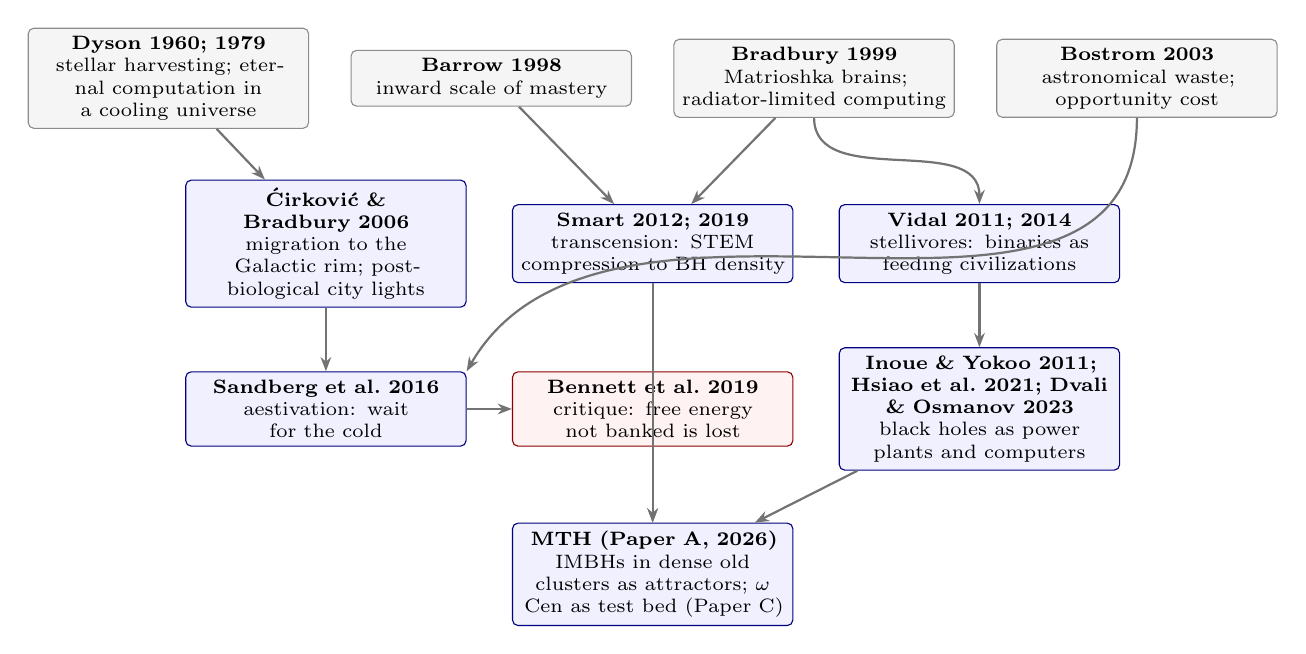
\begin{tikzpicture}[
  era/.style={font=\scriptsize\bfseries, text=black!55},
  box/.style={rectangle, rounded corners=2pt, draw=blue!50!black, fill=blue!6, text width=3.35cm, align=center, font=\scriptsize, inner sep=3pt},
  pre/.style={rectangle, rounded corners=2pt, draw=black!45, fill=black!4, text width=3.35cm, align=center, font=\scriptsize, inner sep=3pt},
  crit/.style={rectangle, rounded corners=2pt, draw=red!55!black, fill=red!5, text width=3.35cm, align=center, font=\scriptsize, inner sep=3pt},
  arr/.style={-{Stealth[length=1.8mm]}, thick, black!55}
]
\node[pre] (dyson) at (0,0) {\textbf{Dyson 1960; 1979}\\ stellar harvesting; eternal computation in a cooling universe};
\node[pre] (barrow) at (4.1,0) {\textbf{Barrow 1998}\\ inward scale of mastery};
\node[pre] (bradbury) at (8.2,0) {\textbf{Bradbury 1999}\\ Matrioshka brains; radiator-limited computing};
\node[pre] (bostrom) at (12.3,0) {\textbf{Bostrom 2003}\\ astronomical waste; opportunity cost};
\node[box] (cirkovic) at (2.0,-2.1) {\textbf{\'Cirkovi\'c \& Bradbury 2006}\\ migration to the Galactic rim; postbiological city lights};
\node[box] (smart) at (6.15,-2.1) {\textbf{Smart 2012; 2019}\\ transcension: STEM compression to BH density};
\node[box] (vidal) at (10.3,-2.1) {\textbf{Vidal 2011; 2014}\\ stellivores: binaries as feeding civilizations};
\node[box] (sandberg) at (2.0,-4.2) {\textbf{Sandberg et al.\ 2016}\\ aestivation: wait for the cold};
\node[crit] (bennett) at (6.15,-4.2) {\textbf{Bennett et al.\ 2019}\\ critique: free energy not banked is lost};
\node[box] (bh) at (10.3,-4.2) {\textbf{Inoue \& Yokoo 2011; Hsiao et al.\ 2021; Dvali \& Osmanov 2023}\\ black holes as power plants and computers};
\node[box] (mth) at (6.15,-6.3) {\textbf{MTH (Paper A, 2026)}\\ IMBHs in dense old clusters as attractors; $\omega$ Cen as test bed (Paper C)};
\draw[arr] (dyson) -- (cirkovic);
\draw[arr] (barrow) -- (smart);
\draw[arr] (bradbury) -- (smart);
\draw[arr] (bradbury.south) to[out=-90,in=90] (vidal.north);
\draw[arr] (bostrom.south) to[out=-90,in=60] (sandberg.north east);
\draw[arr] (cirkovic) -- (sandberg);
\draw[arr] (sandberg) -- (bennett);
\draw[arr] (smart) -- (mth);
\draw[arr] (bennett) -- (mth);
\draw[arr] (bh) -- (mth);
\draw[arr] (vidal) -- (bh);
\end{tikzpicture}
\caption{The inward-family lineage. Grey: precursors that supplied components without stating a Fermi solution. Blue: family members reviewed in Section~\ref{sec:family}. Red: the pivotal critique. Arrows indicate intellectual descent, documented by citation or explicit response where verifiable and thematic otherwise; in particular the stellivore~$\to$~black-hole-computing arrow is thematic, since \citet{Inoue2011} predates \citet{Vidal2014} and does not cite \citet{Vidal2011}.}
\label{fig:tree}
\end{figure}

\subsection{Precursors: Dyson, Barrow, Bradbury, Bostrom}
\label{sec:precursors}

Four threads predate any explicit inward Fermi solution. \citet{Dyson1960} made energy harvesting at stellar scale thinkable and, crucially for everything after, made waste heat the universal observable. \citet{Dyson1979} then showed that computation in an open, cooling universe is in principle unbounded if clock rates slow with the ambient temperature: the first rigorous treatment of computation as the long-run currency of intelligence, later sharpened against $\Lambda$-dominated expansion, which imposes a finite total \citep{KraussStarkman2000}. \citet{Barrow1998} formalized the inward axis itself, ranking civilizations by mastery of ever-smaller scales as a complement to the Kardashev energy scale \citep{Kardashev1964}. \citet{Bradbury1999} engineered the first concrete inward artifact, the Matrioshka brain, and discovered its binding constraint: nested shells are limited by radiator area and sink temperature rather than by energy supply, the constraint that later black-hole proposals dissolve. Two further objections now stand against the Bradbury lineage as engineering: swarm-element stability requires active stationkeeping against radiation pressure and perturbations \citep{Wright2020}, and \citet{Lacki2025Cascade} shows that Kardashev~II megaswarms are destroyed by collisional cascades on timescales short compared to the occupation times the hypotheses require, unless continuously policed. Any inward proposal that routes through Matrioshka-style construction inherits both. \citet{Bostrom2003}, from philosophy, supplied the economic frame: every century of delayed colonization forgoes a fixed, irrecoverable harvest of free energy, an argument that cuts against waiting strategies and therefore sits in productive tension with aestivation, as \citet{Bennett2019} would later make rigorous.

\subsection{\'Cirkovi\'c \& Bradbury (2006): the migration hypothesis}

\emph{Claim.} Advanced civilizations are postbiological and migrate to the Galactic outskirts, where low temperatures favour efficient computing; SETI fails because it searches the wrong place (inner Galaxy, habitable zones) for the wrong thing (biological-era beacons) \citep{CirkovicBradbury2006}.
\emph{Mechanism.} The same Landauer logic as Section~\ref{sec:sinks}, applied radially across the Galaxy: ambient temperature falls with galactocentric radius.
\emph{Predicted sky.} ``City lights'' at the rim: low-temperature infrared structures in the outer Galaxy; silence in the traditional SETI bands.
\emph{Objections.} The radial temperature gradient is shallow --- the CMB floor of 2.7~K applies everywhere, so the rim's advantage over the solar neighbourhood is a factor of order unity, not the $10^{12+}$ available from horizon sinks; and the observational bind is real at both ends: structures radiating near the achievable 3--10~K floor peak at 300--1000~$\mu$m, outside the WISE bands entirely, so cold-end constraints require far-infrared or submillimetre surveys that have not been performed, while only the warm ($\gtrsim$30~K) end of the predicted population falls within WISE-class sensitivity, where it has been neither sought as a targeted population nor found serendipitously \citep{Wright2014b,Griffith2015}.
\emph{Status.} Untested as stated, but its premise survives intact in every later member; historically the first explicit ``wrong place, wrong observable'' Fermi solution grounded in computation thermodynamics.

\subsection{Smart (2012; 2019): the transcension hypothesis}

\emph{Claim.} The developmental trajectory of complexity, ``STEM compression'' of space, time, energy, and matter, carries every sufficiently advanced intelligence toward black-hole-density confinement and, ultimately, out of the observable universe; the silence is a developmental constant, not a contingency \citep{Smart2012,Smart2019}.
\emph{Mechanism.} An evolutionary-developmental analogy: as in ontogeny, the endpoint is convergent and encoded in the dynamics, with black-hole-scale density as the attractor.
\emph{Predicted sky.} Near-total silence; Smart suggests transiting-companion signatures of inner-space civilizations as a long-shot observable.
\emph{Objections.} The terminal step (exit from the universe) invokes physics that is unspecified and untestable in principle --- the standing criticism that motivated the ``macro'' variant (Section~\ref{sec:mth}); the developmental analogy supplies direction but no selection theory over real objects; and the hypothesis as stated cannot be killed by any feasible observation, the cardinal scientific objection.
\emph{Status.} Unfalsifiable as stated (Table~\ref{tab:scorecard}); enormously generative as a research program --- nearly every subsequent member cites it as the frame.

\subsection{Vidal (2011; 2014): stellivores}

\emph{Claim.} Some observed astrophysical systems, specifically accreting binaries, may already be advanced civilizations feeding on stars: ``stellivores.'' The Fermi question is inverted: they are not absent, they are misclassified \citep{Vidal2011,Vidal2014}.
\emph{Mechanism.} Energy logic of accretion (correct, and quantitatively the strongest in the family pre-2023), combined with a cybernetic reading of binary-system regulation.
\emph{Predicted sky.} The X-ray-binary and cataclysmic-variable populations contain technological members distinguishable, if at all, by anomalous regulation statistics.
\emph{Objections.} Standard accretion astrophysics explains the cited phenomenology without remainder, so the proposal carries an extreme parsimony burden; no discriminating statistic separating ``fed'' from ``feeding'' systems has been exhibited; and the claim's retreat to in-principle indistinguishability flirts with unfalsifiability.
\emph{Status.} No proposed test has been carried out; the population-statistics route (regulation anomalies across accreting-binary catalogues) remains open and is the fair test (Section~\ref{sec:program}).

\subsection{Sandberg, Armstrong \& \'Cirkovi\'c (2016): aestivation, and the Bennett--Hanson--Riedel critique}
\label{sec:aestivation}

\emph{Claim.} Computation-maximizers harvest resources now but defer computation to the far future, when the CMB has cooled toward the de Sitter floor and each joule buys up to $\sim10^{30}$ times more erasures; they are dormant now, hence silent \citep{Sandberg2016}.
\emph{Mechanism.} The sink hierarchy of Section~\ref{sec:sinks}, exploited in time rather than in space.
\emph{Predicted sky.} Quiet, resource-conserving infrastructure; suppressed stellar-disruption rates in controlled regions; possibly missing baryons curated against waste.
\emph{Objections.} The decisive one is thermodynamic: \citet{Bennett2019} showed that free energy not collected promptly is irreversibly lost (stars burn regardless), so the optimal policy is aggressive present-epoch harvesting with storage, not dormancy; stored negentropy can be spent at any later epoch at that epoch's efficiency, so waiting confers no advantage over harvesting now and computing later, and storage itself carries only small maintenance costs. The authors' premise that erasure cost dominates the budget is also model-dependent: reversible architectures shift the optimum toward computing early. Aestivation survives only in attenuated form (harvest now, archive-grade computation deferred), at which point its observational predictions collapse into those of its neighbours.
\emph{Status.} The critique is widely accepted; the hypothesis's lasting contributions are the explicit defence policy (which yields its only sharp falsifiable prediction: intervention against entropy-wasting astrophysical processes) and the formalization of the efficiency calculus that the whole family now uses.

\subsection{Black holes as infrastructure: Inoue \& Yokoo, Hsiao et al., Dvali \& Osmanov}
\label{sec:bhinfra}

\emph{Claim(s).} Black holes are the terminal power plants and computers: collectors around accreting supermassive holes \citep{Inoue2011}; Dyson-type harvesting of disk luminosity with computed detectability \citep{Hsiao2021}; and black holes (including manufactured micro holes) as the most efficient quantum information processors, with a predicted high-energy neutrino signature from their evaporation \citep{Dvali2023}.
\emph{Mechanism.} Kerr accretion efficiency (5.7--42 per cent of rest mass; \citealt{BardeenPressTeukolsky1972,NovikovThorne1973}), Blandford--Znajek spin extraction \citep{BlandfordZnajek1977,Tchekhovskoy2011}, and horizon-saturated information physics.
\emph{Predicted sky.} \citet{Hsiao2021}: anomalous-SED point sources, a hot inner edge with missing outer disk. \citet{Dvali2023}: burst-mode TeV--PeV neutrinos from compact sky regions, a genuinely novel observable since natural sources do not readily mimic it. The micro-hole channel inherits a live controversy over whether radiation-collapse manufacturing is blocked by Schwinger pair production \citep{AlvarezDominguez2024,Loeb2024Comment}.
\emph{Objections.} None of these works selects which black holes are preferred (the selection problem); the SMBH orientation of \citet{Inoue2011} ignores the hazard and competition profile of galactic nuclei; detectability claims assume the civilization tolerates conspicuous luminosity, in tension with the efficiency motives that brought it there; and the horizon-as-sink accounting inherits the radiator-temperature objection of Section~\ref{sec:sinks}: absent an architecture that radiates near $T_{\rm H}$, the effective erasure cost is set by the machine's own operating temperature, not the horizon's.
\emph{Status.} The \citet{Dvali2023} neutrino channel is the family's most testable near-term prediction and is now the subject of a proposed dedicated monitoring program at a named target \citep{Swanson2026Campaign}; the high-energy SETI frame is surveyed by \citet{Lacki2025}, and the Dyson Minds workshop \citep{Curtis2026DysonMinds} has since developed the observational agenda for the supermassive-host case, recommending anomaly-detection mining of WISE, JWST, and EHT archives.

\subsection{The Macro Transcension Hypothesis (2026)}
\label{sec:mth}

\emph{Claim.} The inward trajectory halts at a macroscopic, observable destination: rapidly spinning IMBHs embedded in dense, old, low-luminosity stellar systems, selected by a four-axis gradient (energy per unit fuel, entropy disposal, storage density, clock-rate control); migration and operation are electromagnetically quiet; Omega Centauri is the highest-ranked accessible target (Paper A).
\emph{Mechanism.} The full Section-\ref{sec:thermo} stack, plus a selection theory over real objects: intermediate mass (storage and erasure advantages saturate at $10^{4\text{--}5}\,\msun$ while hazards grow), high spin (extractable energy), dense old clusters (fuel, stability, uncontested claim).
\emph{Predicted sky.} Silence plus residues: anomalously high spin on gas-starved IMBHs; suppressed accretion relative to ambient supply; secular core depletion; possibly Dvali--Osmanov neutrino bursts. Six instrument-matched tests with pre-registered kill criteria (Paper A, Table 3; operationalized in Paper C).
\emph{Objections} (catalogued at full strength, given the disclosure of Section~\ref{sec:intro}): it inherits the optimization-pressure premise unargued (Section~\ref{sec:problems}); the staged architecture presupposes goal stability over $10^{8}$~yr; the flagship target's IMBH is itself contested ($\lesssim 6\times10^{3}\,\msun$ timing bound versus $\geq 8.2\times10^{3}\,\msun$ kinematic bound; \citealt{BanaresHernandez2025,Haberle2024Nature}; the latest joint MeerKAT--Parkes pulsar timing, spanning 2021--2025, is insensitive to an IMBH of $10^{3}$--$10^{4}\,\msun$ and constrains the central mass only to $<10^{5}\,\msun$ at 90\% confidence, \citealt{ColomiBernadich2026}, leaving the tension unresolved); the class-level retreat (47~Tuc, M54, extragalactic nuclei) risks unfalsifiability-by-relocation, partially bound by the stated class prediction (no Galactic cluster IMBH with $\astar \gtrsim 0.9$ falsifies it for the Milky Way); its erasure-cost advantage rests on the contested horizon-as-sink accounting of Section~\ref{sec:sinks}, which stands against the MTH at the same strength as against the black-hole-computing thread; and the spin residue, its sharpest discriminator, waits on LISA \citep{Babak2017,Colpi2024}.
\emph{Status.} Untested; distinguishable from its relatives chiefly by having purchased falsifiability with named targets, thresholds, and timelines --- the property the scorecard (Section~\ref{sec:comparison}) is designed to price.

% =====================================================================
\section{Comparative analysis}
\label{sec:comparison}

\subsection{The matrix}

Table~\ref{tab:matrix} aligns the family on five axes. Reading across rows reveals the internal disagreements that casual conflation hides: aestivation and transcension disagree about \emph{when} (future versus now); transcension and the MTH disagree about \emph{where} (fabricated density versus existing holes); stellivores and everyone else disagree about \emph{visibility} (already visible versus invisible); and the black-hole-computing thread disagrees with the MTH about \emph{which holes} (supermassive and manufactured-micro versus intermediate).

One asymmetry in the ``core assumption'' column requires disclosure. The MTH row states its premise in weakened subset-form (``a subset of civilizations maximizes computation'') while its competitors are stated in the universal forms their authors used. The subset-form is what Paper A asserts, so the row is accurate, but the weakening buys explanatory cover that the universal forms do not enjoy, and it must be paid for: a subset-form premise faces the incomplete-compliance objection (P4, Section~\ref{sec:problems}) at full strength, since the non-migrating majority still needs explaining, in the same way that a dark forest with imperfect adoption fails as a silence-explanation. Readers comparing rows should either read the competitors charitably in whatever subset-form their authors would accept, or charge the MTH the P4 penalty; the matrix should not be read as granting the newest member a weaker burden.

\begin{table}[tbp]
\centering
\caption{The inward family compared. ``Energy logic'' names the dominant free-energy mechanism; ``appearance'' is the predicted present-epoch sky.}
\label{tab:matrix}
\scriptsize
\begin{tabular}{p{2.2cm}p{2.4cm}p{2.3cm}p{2.6cm}p{2.6cm}p{2.2cm}}
\toprule
Hypothesis & Core assumption & Energy logic & Predicted appearance & Standing objection & Status \\
\midrule
Migration \citep{CirkovicBradbury2006} & postbiological evolution; $T$-sensitive computing & ambient-$T$ Landauer gain at Galactic rim & IR ``city lights'' in outer Galaxy; band silence & rim gain is $\mathcal{O}(1)$, CMB-floored & untested as stated \\
Transcension \citep{Smart2012} & convergent STEM compression & density $\to$ Lloyd-limit computing & near-total silence; transit anomalies & terminal step untestable & unfalsifiable as stated \\
Stellivores \citep{Vidal2014} & some binaries are civilizations & direct stellar accretion & misclassified X-ray binaries & no discriminating statistic offered & open; population test feasible \\
Aestivation \citep{Sandberg2016} & erasure dominates budget; patience & wait for $T_{\rm dS}$: $\sim10^{30}\times$ gain & curated quiet; process suppression & free energy not banked is lost \citep{Bennett2019} & attenuated by critique \\
BH computing \citep{Inoue2011,Hsiao2021,Dvali2023} & holes are optimal processors & Kerr/BZ extraction; horizon information & anomalous SEDs; $\nu$ bursts & no selection theory over holes; radiator-limited sink access (\S\ref{sec:sinks}) & $\nu$ channel newly testable \\
MTH (Paper A) & subset of civilizations maximizes computation & full stack + selection over IMBHs & silence + spin/depletion residues; $\nu$ bursts & optimization premise; goal stability; contested target IMBH; radiator-limited sink access (\S\ref{sec:sinks}) & six pre-registered tests pending \\
\bottomrule
\end{tabular}
\end{table}

\subsection{The falsifiability scorecard}
\label{sec:scorecard}

Table~\ref{tab:scorecard} grades each member against five criteria, fixed before grading: \textbf{C1} -- names a target or target class that observations can interrogate; \textbf{C2} -- states quantitative observables with thresholds; \textbf{C3} -- at least one stated test is executable with existing or funded instruments within $\sim$15 years; \textbf{C4} -- specifies kill conditions in advance (results the proponents agree would refute it); \textbf{C5} -- has survived at least one executed test that could have refuted it. Symbols: \sfull{} met, \shalf{} partially met, \snone{} not met. Three caveats. First, C5 is the column that separates science-in-progress from science-performed: no member of the family scores \sfull{} on C5, because no pre-registered inward-family test has yet been executed to completion; the FAST globular-cluster survey \citep{Huang2026} and the proposed $\omega$~Cen campaign \citep{Swanson2026Campaign} are the first entries in that ledger. Second, given the author's conflict of interest, the MTH row's grades are tied to specific Paper A artifacts rather than to judgement: C1 rests on the named flagship target and ranked fallback class ($\omega$~Cen; 47~Tuc, M54); C2 on the quantitative mass- and spin-constraint table (Paper A, Table 2); C3 on the instrument-matched test schedule against JWST, MeerKAT, Gaia, Roman, and LISA (Paper A, Table 3); and C4 on the six pre-registered kill conditions T1--T6 of that same table. So that these grades are auditable without leaving this paper, the kill conditions include, among others: a LISA spin measurement finding $\astar$ well below the near-extremal band on the flagship IMBH; resolution of the $\omega$~Cen mass tension in favour of an extended dark remnant population rather than a single IMBH; and detection of ordinary accretion variability at the level natural gas supply predicts, which would remove the ``suppressed accretion'' residue. Third, the MTH's strong showing on C1--C4 was purchased after the criteria of falsifiability had been articulated by its predecessors' critics; later entrants always grade better on form, and the scorecard measures testability, not probability of truth.

\begin{table}[tbp]
\centering
\caption{Falsifiability scorecard. Criteria C1--C5 defined in Section~\ref{sec:scorecard}; \sfull{} met, \shalf{} partial, \snone{} not met. The scorecard grades testability, not truth.}
\label{tab:scorecard}
\small
\begin{tabular}{lccccc}
\toprule
Hypothesis & C1 target & C2 thresholds & C3 near-term & C4 kill criteria & C5 survived test \\
\midrule
Migration (2006) & \shalf & \snone & \shalf & \snone & \snone \\
Transcension (2012) & \snone & \snone & \snone & \snone & \snone \\
Stellivores (2011--14) & \sfull & \snone & \shalf & \snone & \snone \\
Aestivation (2016) & \shalf & \shalf & \snone & \sfull & \snone \\
BH computing (2011--23) & \shalf & \shalf & \sfull & \shalf & \snone \\
MTH (2026) & \sfull & \sfull & \sfull & \sfull & \snone \\
\bottomrule
\end{tabular}
\end{table}

Three scorecard judgements require defence. \emph{Aestivation's} \sfull{} on C4 reflects \citet{Sandberg2016}'s explicit and admirable statement of refuting observations (uncontrolled entropy-wasting processes in regions a defender should police); its \snone{} on C3 reflects that no instrument can audit process-suppression statistics at the required scale on any near-term horizon. \emph{Transcension's} row of \snone{} is not a dismissal of its generativity (half the family descends from it) but the direct application of the criteria to a hypothesis whose endpoint is defined as unobservable; \citet{Smart2019} adds developmental argument, not observables. \emph{BH computing's} \sfull{} on C3 is carried entirely by the \citet{Dvali2023} neutrino channel, which named an energy range, a temporal structure, and a source class that current telescopes can monitor \citep{KM3NeT2025,IceCubePS2020}. Finally, the C3 asymmetry between the MTH (\sfull) and aestivation (\snone) is principled rather than partisan: C3 asks whether a stated test is executable with existing or funded instruments within $\sim$15 years, and the MTH's spin test rides on LISA, an adopted and funded mission inside that window \citep{Colpi2024}, whereas aestivation's process-suppression audit has no equivalent funded instrument on any announced schedule.

% =====================================================================
\section{The sociological competitors}
\label{sec:sociological}

Three well-known solutions predict the same silent sky from non-thermodynamic premises, and the family is best understood against them.

\textbf{Zoo \citep{Ball1973} and its hegemony refinement \citep{Forgan2017}.} Silence as policy: we are observed but quarantined. Forgan's contribution is structural --- a zoo requires either a single dominant culture or stable inter-civilization consensus (``Galactic Club''), and fragmented ``cliques'' should leak defectors. The premise is sociological uniformity over megayear timescales, the premise the inward family replaces with physics.

\textbf{Dark forest \citep{Brin1983,Yu2015}.} Silence as survival strategy under first-strike game theory. Its physics is sound (relativistic kill vehicles are cheap; detection is asymmetric), and its deadly-probes mechanism has received technical treatment: \citet{Forgan2019Probes} models mutated ``predator'' probes suppressing a visible probe population with Lotka--Volterra dynamics and finds that stable equilibria typically retain large prey populations, undercutting the mechanism as a full silence-explanation. The equilibrium is also fragile: the strategy must be adopted by every civilization without exception and without deviation forever, since a single loud defector (or a single expansionist willing to absorb risk) breaks the explanatory account \citep{Brin1983,Forgan2017}. Like the zoo, it predicts pure silence: no residue, no test, no scheduled adjudication.

\textbf{Sustainability \citep{HaqqMisraBaum2009}.} Exponential expansion is self-terminating; civilizations that persist are those that grow slowly or not at all. This is the mildest competitor, and partially complementary: it removes the pressure to expand without supplying a positive account of where mature capability is directed.

The comparison clarifies what the inward family is actually claiming. All these proposals, sociological and thermodynamic alike, break the expansionist premise. The differences are two. \emph{Robustness}: dark-forest and zoo equilibria are fragile to a single defector among all civilizations across all time, whereas the inward account requires no coordination at all --- each civilization independently follows its own resource gradient, and partial compliance merely thins the loud population rather than collapsing the explanation (a point made quantitative in the grabby-aliens frame; \citealt{Hanson2021}; see Section~\ref{sec:problems}). \emph{Residue}: fear and policy predict nothing observable, by design; thermodynamic optimization is a physical process operating on physical objects, and physical processes leave traces: spin histories, depletion statistics, suppressed accretion, burst channels. Among the silence-explanations, the inward family is the falsifiable-in-principle wing, and grading its members' falsifiability in practice (Table~\ref{tab:scorecard}) is therefore where a review can add value.

% =====================================================================
\section{Open problems}
\label{sec:problems}

We state the family's unsolved problems as research questions rather than objections, since several are tractable.

\paragraph{P1: The optimization premise.} Every member assumes some civilizations converge on maximizing computation (or a correlate). The premise is defended by universality arguments (computation is the currency into which most terminal goals are convertible; \citealt{Smart2012,Sandberg2016,Bostrom2003}) but it has never been given a selection-theoretic foundation: under what competitive or evolutionary dynamics do computation-maximizers come to exist, persist, and dominate the behaviour of their lineage? The grabby-aliens machinery \citep{Hanson2021,Olson2015} could be adapted to model mixed populations (maximizers, expansionists, satisficers) and derive the observable consequences of each mixture; the companion economics paper supplies a capture term for that machinery but defers the full integration \citep{Swanson2026Economics}.

\paragraph{P2: Goal stability over $10^{8}$ years.} Inward strategies require coherent purpose across timescales exceeding mammalian evolutionary history, flagged as the largest unargued premise even by the family's own proponents (Paper A). The mitigation argument (front-loaded payoffs leave permanent residues even if the lineage fragments mid-program) rescues the observational program but not the hypothesis's interior logic. The family's deepest dependency is therefore a theory of institution or value stability under self-modification, a problem that lies outside astronomy.

\paragraph{P3: Migration economics.} \citet{Bostrom2003}'s opportunity-cost argument prices delay; \citet{Bennett2019} price dormancy; nobody has priced relocation. The trade is concrete: a migrating lineage abandons its accumulated local infrastructure for transit times of $10^{4\text{--}6}$~yr in exchange for a destination whose advantages (Section~\ref{sec:thermo}) are enormous but deferred. Under what discount rates, risk models, and replication strategies does migration dominate local densification (Matrioshka-style; \citealt{Bradbury1999})? This is a well-posed optimization problem, and it has since received a first quantitative treatment in a companion paper \citep{Swanson2026Economics}, which derives closed-form crossover thresholds among staying, migrating, and seed-dispatch strategies. We retain the problem in this list because the treatment's inputs (discount and hazard rates over agents never observed) remain open, and because its population-level corollaries feed directly into P4.

\paragraph{P4: Incomplete compliance.} If migration is optional, the loud expansionists we do not see still need explaining. The defensible position (argued in Paper A) is that inward migration thins the expected loud population by removing its most capable members, sharpening rather than dissolving the paradox; full dissolution requires either high compliance or supplementary rarity from conventional Drake factors. Quantifying ``how much thinning suffices'' against the \citet{Hanson2021} selection effect is open problem P1's observational face.

\paragraph{P5: Degeneracy of silence.} $H_0$-type explanations (gas starvation, rarity) and inward-family explanations predict identical electromagnetic appearances; only residues discriminate. The family therefore lives or dies on the residue catalogue (spin, depletion, bursts, regulation statistics), and enlarging that catalogue with new discriminators is the highest-leverage theoretical work available. The contested micro-black-hole manufacturing channel \citep{AlvarezDominguez2024,Loeb2024Comment} is a case in point: it would be a sharp discriminator if the manufacturing route is physical, and it drops out of the catalogue if Schwinger pair production blocks it.

% =====================================================================
\section{The observational program}
\label{sec:program}

The family is no longer untestable in practice; Table~\ref{tab:tests} maps each member to its executable tests. Four clusters of activity dominate.

\begin{table}[tbp]
\centering
\caption{Instrument-matched tests of the inward family, 2026--2040. Status: A = archival/feasible now; P = proposed; F = free by-product of funded missions.}
\label{tab:tests}
\scriptsize
\begin{tabular}{p{2.6cm}p{3.6cm}p{3.0cm}p{1.2cm}p{3.0cm}}
\toprule
Hypothesis & Test & Instrument(s) & Status & Refutes / constrains \\
\midrule
Migration (rim) & targeted IR census of outer-Galaxy low-$T$ structures & WISE/JWST archival; Roman & A & rim ``city lights'' population \\
Stellivores & regulation-anomaly statistics across accreting-binary catalogues & X-ray archives (Chandra, XMM, eROSITA) & A & ``feeding'' vs ``fed'' discrimination \\
Aestivation (attenuated) & process-suppression statistics in old quiescent systems & survey archives; LSST & A & curated-region prediction \\
BH computing ($\nu$) & burst-mode TeV--PeV multiplets from candidate sites & KM3NeT/ARCA, IceCube & P & \citet{Dvali2023} channel at stated strength \\
MTH & six pre-registered tests at $\omega$ Cen: accretion/waste-heat limits, timing profile, astrometry, spin & JWST, MeerKAT/SKA, Roman, Gaia, LISA & P/F & kill criteria T1--T6 of Paper A \\
Family-wide & waste-heat nulls at increasing depth & \^G successors; Gaia Dyson candidates & A & expansionist premise (control) \\
Family-wide & GC technosignature surveys & FAST \citep{Huang2026}; MeerKAT & A/P & first dedicated old-population SETI \\
\bottomrule
\end{tabular}
\end{table}

\textbf{(i) Globular clusters as the family's natural laboratory.} Old, dense, dynamically relaxed, electromagnetically quiet, and, for the IMBH-hosting subset, equipped with the objects the gradient selects. The FAST pilot survey \citep{Huang2026} opened the niche, and Gaia-based dynamical-extremeness metrics now exist for ranking clusters as technosignature targets \citep{Huang2026Crystallization}; the $\omega$~Cen multi-messenger campaign (Paper C) is the first program designed end-to-end around inward-family falsification, with the conventional astrophysics (the IMBH mass tension; \citealt{Haberle2024Nature,BanaresHernandez2025}) guaranteeing scientific value under every outcome. That tension remains live: the latest joint MeerKAT and Parkes timing of the cluster's millisecond pulsars (2021--2025) is insensitive to an IMBH in the contested $10^{3}$--$10^{4}\,\msun$ range and bounds the central mass only from above, at $<10^{5}\,\msun$ at 90\% confidence \citep{ColomiBernadich2026}, so the timing--kinematics discrepancy awaits deeper data. The cluster's compact-object inventory has meanwhile begun to resolve directly: 23 years of HST and JWST astrometry have yielded the first stellar-mass black hole detected astrometrically in any globular cluster, the $4.46\,\msun$ oMEGACat BH-2 in a 94-yr binary \citep{Whitaker2026BH2}, the first confirmed member of the $\sim$$10^{4}$ stellar-mass black holes that dynamical models of the cluster predict \citep{Zocchi2019,BreenHeggie2013}.

\textbf{(ii) The spin channel.} Among all residues, black-hole spin is unique: permanent, quantitative, and measurable to $\sim10^{-3}$ precision by LISA for favourable systems \citep{Babak2017,AmaroSeoane2018,Colpi2024}. A near-extremal spin on a demonstrably gas-starved IMBH has no comfortable natural history; a low spin retires the exploitation models outright. No other proposed technosignature combines this permanence with a funded instrument.

\textbf{(iii) The neutrino channel.} The \citet{Dvali2023} burst phenomenology is testable now at named targets with operating instruments \citep{KM3NeT2025,AntaresIceCube2020}; the pre-registered multiplet criteria are specified in Paper C. A decade-scale null closes the channel at its stated strength.

\textbf{(iv) Population statistics over single objects.} For stellivores and attenuated aestivation, the executable tests are statistical: regulation anomalies across binary catalogues; suppression statistics across old systems. These reuse public archives, cost salaries only, and would convert the family's two least-tested members from rhetoric to results.

The program has a unifying property: every test doubles as conventional astrophysics (IMBH demographics, accretion physics, binary populations, cluster dynamics), so the field can pursue the family's adjudication without betting careers on its truth. The pattern is inherited from the waste-heat surveys \citep{Wright2014,Griffith2015} and from the falsificationist turn of \citet{Sandberg2016} and \citet{Dvali2023}, and it holds whatever the individual hypotheses' fates.

% =====================================================================
\section{Conclusion}
\label{sec:conclusion}

Reviewed as a family, the inward hypotheses form a six-decade research lineage with a common physical premise, the thermodynamics of computation as the lens for predicting mature intelligence, and genuine internal disagreements about timing, destination, and visibility that observation can, increasingly, adjudicate. The family's intellectual trajectory is itself instructive: from direction without destination (\'Cirkovi\'c \& Bradbury), through destination without testability (transcension), through testability purchased by critique (aestivation and its Bennett--Hanson--Riedel correction), to the current generation's explicit targets, thresholds, and kill criteria. Each generation's advance was forced by the previous generation's sharpest critics.

Against the sociological silence-solutions, the family's distinguishing asset is residue: physics leaves traces where policy does not. Its distinguishing liability is the optimization premise, which remains unargued at the selection-theoretic level where it would need to be argued (open problem P1). Between asset and liability sits the practical situation of 2026: for the first time, members of this family have pre-registered tests scheduled on funded instruments, anchored by the globular-cluster surveys now beginning and by LISA's spin measurements a decade out. Within fifteen years the scorecard's empty C5 column will have entries. Whatever they say, the column will no longer be empty --- which is, for a literature long accused of unfalsifiability, the most consequential outcome.

% =====================================================================
\section*{Acknowledgements and disclosure}

The author thanks the maintainers of the NASA Astrophysics Data System and arXiv, on which the citation verification for this work relied. The author's conflict of interest as proponent of one reviewed hypothesis is disclosed in Section~\ref{sec:intro} and mitigated by the fixed-criteria comparative method of Section~\ref{sec:comparison}. \textbf{AI assistance disclosure:} drafting, citation verification, derivation checking, and figure preparation for this manuscript were performed with substantial assistance from a large language model (Claude, Anthropic), under the author's direction; the author reviewed and takes full responsibility for all claims, derivations, and references. Interactive calculators implementing the quantitative material in Section~\ref{sec:thermo} are available at \url{https://omegacentauri.me}.

\section*{Data availability}

No new observational data were generated for this work. All quantitative claims derive from the cited literature.

\bibliographystyle{apalike}
\bibliography{references,campaign-extra,inward-extra}

\end{document}
